\documentclass[11pt]{article}
\usepackage{tikz}
\usetikzlibrary{shapes, arrows}
\usepackage[hmargin=1in,vmargin=1in]{geometry}
\usepackage{xcolor}
\usepackage{enumitem} 
\usepackage{wrapfig}
\usepackage{amsmath,amssymb,amsfonts,url,sectsty,framed,tcolorbox,framed}
\newcommand{\pf}{{\bf Proof: }}
\newtheorem{theorem}{Theorem}
\newtheorem{lemma}{Lemma}
\newtheorem{proposition}{Proposition}
\newtheorem{definition}{Definition}  
\newtheorem{remark}{Remark}
\newcommand{\qed}{\hfill \rule{2mm}{2mm}}
\usepackage{fixltx2e}
\usepackage{graphicx}
\newcommand*{\xdash}[1][3em]{\rule[0.5ex]{#1}{0.55pt}}
\begin{document}
	\noindent
	\rule{\textwidth}{1pt}
	\begin{center}
		{\bf [CS304] Introduction to Cryptography and Network Security}
	\end{center}
	Course Instructor: Dr. Dibyendu Roy \hfill Winter 2022-2023\\
	Scribed by : Pallikonda Sai Teja  \hfill Lecture (Week 05)\\
	Student ID : 202011052\\
	\rule{\textwidth}{1pt}
	\section{Group}
	$\bullet$ Group $\rightarrow$ (G,$\ast$) \hfill 
	\begin{tabular}{| c |}
		\hline
		G is closed under $\ast$\\
		\hline
	\end{tabular}\\
	$\alpha \in$ G\\
	$\alpha^0, \alpha^1, \alpha^2,... \in$ G\\
	$\alpha^0 \rightarrow$ identity\\
	for a b $\in$ G\\
	$\exists$ i $\geq$ such that b = $\alpha^i$ $\Rightarrow$ G $\subseteq$ $<\alpha>$\\
	then $\alpha$ is called the generator of (G, $\ast$)\\
	$\bullet$ (G, $\ast$) = $<\alpha>$\\
	$\bullet$ A Group G is cyclic if there is an element $\alpha \in$ G, such that for every b $\in$ G there is an integer i with b = $\alpha^i$\\
	This $\alpha$ is called the generator of G. $$G = <\alpha>$$
	$\bullet$ (G, $\ast$) \hfill $|G|$ : finite\\
	a $\in$ G o(a) = m, $a^m$ = e\\
	e = $a^0, a^1, a^2,..,a^{m-1} in$ G\\
	H = \{$a^0, a^1, a^2,..,a^{m-1}$\}
	\begin{enumerate}
		\item H  $\subseteq$ G
		\item H is a group under $\ast$\\if x, y $\in$ H\\$\Rightarrow$ x $\ast$ y $\in$ H
	\end{enumerate}
	for every $a^i$ $\in$ H $\exists$ the inverse of $a^i$\\
	H is a group with $\ast$.\\
	H is a sub group of G.$$H = <a>$$
	H is a cyclic sub group of G.\\
	$|H|$ = $|<a>|$ $\rightarrow$ order of cyclic subgroup = O(a)
	
	\section{Lagrange Theorem}
	If G is a finite group.\\
	H is a sub group of G then $|H|$ divides $|G|$.\hfill 
	\begin{tabular}{| c |}
		\hline
		$|S|$ is cardinality of set S\\
		\hline
	\end{tabular}\vspace{0.3cm}\\
	$\bullet$ G is a finite group \\
	a $\in$ G\\
	O(a) divides $|G|$.\\
	$rightarrow$ a $\in$ G\\
	H = \{e=$a^0, a^1, a^2,.., a^{O(a)-1}$\}\\
	H is a sub group of G.\vspace{0.3cm}\\
	$\bullet$ If the order of a $\in$ G is t then $$O(a) = \frac{t}{gcd(t,k)}$$
	If gcd(t, k) = 1\\
	then O($a^k$) = t = O(a)\\
	$\Rightarrow$ $|<a^k>|$ = $|<$a$>|$\\
	x $\in$ $<a^k>$\\
	$\Rightarrow$ x = $(a^k)^i$ = $a^{ki}$ $\in$ $<$a$>$ \\
	$<a^k>$ $\subseteq$ $<$a$>$\\
	$<a^k>$ = $<$a$>$ \hfill ( Since $|<a^k>|$ = $|<$a$>|$ )\\
	$a^k$ is also a generator of $<a>$\vspace{0.3cm}\\
	$\bullet$ ${Z^{\ast}}\textsubscript{19}$ = \{ x $|$ gcd(x, 19) = 1, 1 $\leq$ x $\leq$ 18 \}\\
	$\ast\textsubscript{19}$ : multiplication modulo 19.\vspace{0.3cm}\\
	Find the generator of (${Z^{\ast}}\textsubscript{19}$, $\ast\textsubscript{19}$)\\
	$<2>$ =\{1, 2, 4, 8, 16, 13, 7, 14, 9, 18, 17, 15, 11, 3, 6, 12, 5, 10\} = ${Z^{\ast}}\textsubscript{19}$\\
	$<2^5>$ = $<13>$ is also a generator of ${Z^{\ast}}\textsubscript{19}$\\
	
	\section{Ring}
	A ring (R, +\textsubscript{R}, $\ast$\textsubscript{R}) consists of one set R with two binary operations arbitrarily denoted by +\textsubscript{R} (addition) and $\ast$\textsubscript{R} (multiplication) on R satisfing the following properties.
	\begin{enumerate}
		\item (R, +\textsubscript{R}) is a abelian group with the identity element 0\textsubscript{R}.
		\item The operation $\ast$\textsubscript{R}) is associate i.e., $$a\ast\textsubscript{R}(b\ast\textsubscript{R}c) = (a\ast\textsubscript{R}b)\ast\textsubscript{R}c\hspace{0.2cm} \forall\hspace{0.1cm} a,b,c \in R$$
		\item There is a multiplication identity denooted by 1\textsubscript{R} with 1\textsubscript{R} $\neq$ )\textsubscript{R} such that $$1\textsubscript{R}\ast\textsubscript{R}a = a\ast\textsubscript{R}1\textsubscript{R} = a\hspace{0.2cm} \forall\hspace{0.1cm} a \in R$$
		\item The operation $\ast$\textsubscript{R} is distributive over +\textsubscript{R} i.e.,$$(b+\textsubscript{R}c)\ast\textsubscript{R}a = (b\ast\textsubscript{R}a)+\textsubscript{R}(c\ast\textsubscript{R}a)$$
		$$a\ast\textsubscript{R}(b+\textsubscript{R}c) = (a\ast\textsubscript{R}b)+\textsubscript{R}(a\ast\textsubscript{R}c)$$
	\end{enumerate}
	Example : (Z, +, .) $\rightarrow$ Ring\\
	$\Rightarrow$ a.b = b.a $\forall$ a, b $\in$ Z commutative ring \\
	An element 'a' of a ring R is called unit or an invertable elements if there is an element b $\in$ R such that a $\ast$\textsubscript{R}b = 1\textsubscript{R}\\
	$\bullet$ The set of units in a Ring R forms a group under multiplication operation.\\
	$\Rightarrow$ This is known as group of units of R.
	
	
	
	\section{Field}
	A field is a non-empty set F together with two binary operations +(addition) and $\ast$(multiplication) for which the following properties are satisfied.
	\begin{enumerate}
		\item (F, +) is an abelian group.
		\item If 0\textsubscript{F} denotes the additive identity element of (F,+) then (F $\backslash$ \{0\textsubscript{F}\}, $\ast$) is a commutative abelian group.
		\item $\forall$ a, b, c $\in$ F we have
		$$ a*(b+c) = (a*b) + (a*c)$$
	\end{enumerate}
	
	Example: (Z\textsubscript{P},+\textsubscript{P},$\ast$\textsubscript{P}) $\rightarrow$ Field ? \hfill P$\rightarrow$ Prime
	\begin{enumerate}
		\item Z\textsubscript{P} = \{0,1,2,...,P-1\}
		\item It is a group under first operation.
		\item 0 is the identity, if x $\in$ Z\textsubscript{P} then $\exists$ P-x such that x +\textsubscript{P} (P-x) = 0.
		\item The operation is commutative.
		\item (\{Z\textsubscript{P - 0}\}, $\ast$) is a commutative group.
		\item $\exists$ multiplicative identity is "1".
		\item x $\in$ \{Z\textsubscript{P}-0\} $\exists$ y $\in$ \{Z\textsubscript{P}-0\} such that x $\ast$\textsubscript{P}
		y = 1, because (x, p) = 1.
		\item It is a abelian group. $$ x \ast y mod p = y \ast x mod p.$$
		\item It is distributive $$ a \ast \textsubscript{P}(b +\textsubscript{p} c = ( a \ast\textsubscript{p}  b) +\textsubscript{p} ( a \ast\textsubscript{p}  c) $$
		$$ (Z\textsubscript{P}, +\textsubscript{P}, \ast \textsubscript{P}) \rightarrow Field$$ 
		
	\end{enumerate}
	
	\section{Field Extension}
	Suppose k\textsubscript{2} is a field with addition (+) and multiplication (*). Suppose k\textsubscript{1} $\subseteq$ k\textsubscript{2} is closed under both these operations such that k\textsubscript{1} itself is a field with the restriction of + and * the set k\textsubscript{1}.\vspace{0.3cm}\\
	$\bullet$ F $\rightarrow$ field (F, +, $\ast$)\\
	F(x) = \{a\textsubscript{0} + a\textsubscript{1}x + ...$|$ a\textsubscript{i} $\in$ F\}\hfill
	(F(x), +, $\ast$) $\rightarrow$ Polynomial Ring\\
	+ $\rightarrow$ Polynomial addition\\
	$\ast \rightarrow$ Polynomial multiplication\\
	P\textsubscript{1}(x) $\in$ F(x), P\textsubscript{1}(x) = a\textsubscript{0} + a\textsubscript{1}x + a\textsubscript{2}$x^2$\\
	P\textsubscript{2}(x) $\in$ F(x), P\textsubscript{2}(x) = b\textsubscript{0} + b\textsubscript{1}x + b\textsubscript{2}$x^2$\\
	P\textsubscript{1}(x) + P\textsubscript{2}(x) = (a\textsubscript{0} + a\textsubscript{1}x + a\textsubscript{2}$x^2$) + (b\textsubscript{0} + b\textsubscript{1}x + b\textsubscript{2}$x^2$)\\
	P\textsubscript{1}(x) + P\textsubscript{2}(x) = (a\textsubscript{0} + b\textsubscript{0}) + (a\textsubscript{1} + b\textsubscript{1})$x$ + (a\textsubscript{2} + b\textsubscript{2})$x^2$\\
	(a\textsubscript{i} + b\textsubscript{i}) $\rightarrow$ Field addition.\\
	additive operation on F as (a\textsubscript{i}, b\textsubscript{i}) $\in$ F.\\
	$\rightarrow$ (a\textsubscript{0} + a\textsubscript{1}x + a\textsubscript{2}$x^2$ + .. + a\textsubscript{n-1}$x^{n-1}$) $\ast$ (b\textsubscript{0} + b\textsubscript{1}x + b\textsubscript{2}$x^2$ + .. + b\textsubscript{n-1}$x^{n-1}$)\\
	= a\textsubscript{0}b\textsubscript{0} + (a\textsubscript{0}b\textsubscript{1} + a\textsubscript{1}b\textsubscript{0})$x$ +....+ (a\textsubscript{n-1}b\textsubscript{n-1})$x^{2n-2}$\\
	a\textsubscript{i} $\ast$ b\textsubscript{i} $\rightarrow$ Field multiplication in F as a\textsubscript{i}, b\textsubscript{i} $\in$ F.\\
	addition between the elements has to be done in the field.\\
	$\bullet$ (F[x], +, $\ast$) is a polynomial ring.\\
	\begin{enumerate}
		\item (F[x], +) must be a abelian group.\\
		\hspace*{0.4cm}a\textsubscript{0} + a\textsubscript{1}x + a\textsubscript{2}$x^2$\hfill a\textsubscript{i} $\in$ F\\
		+ b\textsubscript{0} + b\textsubscript{1}x + b\textsubscript{2}$x^2$\hfill a\textsubscript{i} + b\textsubscript{i} = 0\\\hspace*{0.2cm} \xdash[7.8em]\\
		\hspace*{0.4cm}(a\textsubscript{0} + b\textsubscript{0}) + (a\textsubscript{1} + b\textsubscript{1})$x$ + (a\textsubscript{2} + b\textsubscript{2})$x^2$ = 0
		\item $\ast$ is associative.
		\item 1 is the multiplicative identity.
		\item $\ast$ is distributive over +.
	\end{enumerate}
	$\bullet$ F\textsubscript{2} = \{0,1\} \hfill (F\textsubscript{2}, +\textsubscript{2}, $\ast$\textsubscript{2}) $\rightarrow$ Field\\
	F\textsubscript{2}[x] = \{a\textsubscript{0} + a\textsubscript{1}x + a\textsubscript{2}$x^2$+...
	$|$ a\textsubscript{i} $\in$ F\textsubscript{2}\}\\
	p(x) = x + 1     $\in$ F\textsubscript{2}[x]\\
	q(x) = $x^2$+x+1    $\in$ F\textsubscript{2}[x]\\
	p(x) + q(x) =  (x + 1) + ($x^2$ + x + 1)= $x^2$ + (1+1)x + (1+1)= $x^2$
	p(x) $\ast$ q(x) = (x+1)$\ast$($x^2$+x+1) = ($x^3$ + $x^2$+ x) + ($x^2$+x+1) = $x^3$ +(1+1)$x^2$ + (1+1)x + 1 = $x^3$ + 1.\vspace{0.3cm}\\
	$\bullet$ A polynomial P(x) $\in$ F(x) of degree n (n $>=$ 1) is called irreduciable if it cannot be written in the form of 
	P\textsubscript{1}(x)$\ast$ P\textsubscript{2}(x) with P\textsubscript{1}(x), P\textsubscript{2}(x) $\in$ F[x]
	and degree of P\textsubscript{1}(x), P\textsubscript{2}(x) must be $>=$ 1.\\
	$$P(x) \neq P\textsubscript{1}(x)\ast P\textsubscript{2}(x)$$.\\
	$\bullet$ $x^2$ + 1 $\in$ F(x) \\
	(x+1)$\ast$(x+1) = $x^2$+(1+1)x+1 = $x^2$ + 1.\\
	($x^2$ + 1) = (x+1)$\ast$ (x+1) in F\textsubscript{2}[x]\\
	$x^2$ + 1 is reducable in F\textsubscript{2}[x]\vspace{0.3cm}\\
	$\bullet$ I = $<P(x)>$ = \{Q(x).P(x) $|$ Q(x) $\in$ F(x)\} \\
	I $\rightarrow$ ideal generated by P(x).\vspace{0.3cm}\\
	$\bullet$ f[x] / $<P(x)>$ = \{g(x) \% P(x) $|$ g(x) $\in$ F(x)\}\\
	Q(x) $\in$  F[1] \\
	Q(x) = d(x) $\ast$ P(x) $\ast$ r(x) \\
	r(x) $\in$ F[x]$/$$<P(x)>$\\
	if P(x) is irreducable polynomial then
	
	(F[x]/$<P(x)>$, +, $\ast$) becomes field.\\
	Example : $x^2 + x + 1 \in $ F\textsubscript{2}[x], F\textsubscript{2} = \{0, 1\}\\
	P(x) = $x^2 + x + 1$ is irreducible \vspace{0.3cm}\\
	$\bullet$ F\textsubscript{2}[x]/$<x^2 + x + 1>$\\
	q(x) = d(x).p(x) + r(x)\\
	deg(r(x)) $<$ 2\\
	r(x) = \{0, 1, x, x+1\}\vspace{0.3cm}\\
	$\bullet$ $x^2 + x + 1$ ) $x^2 + 1$ ( 1\\
	\hspace*{2cm} $x^2 + x + 1$\\
	\hspace*{2cm} \xdash[5em]\\
	\hspace*{2.7cm} $x$\vspace{0.3cm}\\
	$\bullet$ $x^3 + 1$\\
	= $x.x^2 + 1$\\
	= $x(x + 1) + 1$\\
	= $x^2 + x + 1$\\
	= $x + 1 + x + 1$\\
	= 0\vspace{0.3cm}\\
	$\bullet$ F\textsubscript{2}[x] / $<x^2 + x + 1>$\\
	$x^2 + x + 1$ = 0\\
	$\alpha$ is the root of $x^2 + x + 1$ = 0\\
	$\alpha^2 + \alpha + 1 = 0$\\
	$\Rightarrow$ $\alpha^2 = \alpha + 1$\\
	$<\alpha>$ = \{0, 1=$\alpha^0$, $\alpha^1$, $\alpha^2 = \alpha + 1$\} $\Rightarrow$ O($\alpha$) = 2\\
	$\Rightarrow$ \{0, 1, $\alpha$, $\alpha + 1$\}\\
	$x^2 + x + 1$ is a primitive polynomial.\vspace{0.3cm}\\
	Example : F\textsubscript{2}[x] / $<x^3 + x + 1>$\\
	=\{$0, 1, x, x + 1, x^2, x^2+1, x^2+x, x^2+x+1$\}\\
	$\alpha^3 + \alpha + 1 = 0$\\
	$\alpha^3 = \alpha + 1$\\
	\{$0, \alpha, \alpha^2, \alpha^3 = \alpha+1, \alpha^2+\alpha, \alpha^2+\alpha+1, \alpha^2+1, 1$\}\\
	$x^3 + x + 1$ is a primitive polynomial.\\
	$x^2 * (x^2 + x + 1)$ = $x^4 + x^3 + x^2$\\
	= $x(x+1) + (x+1) + x^2$\\
	= $x^2 + x + x + 1 + x^2$\\
	= 1
	
	\section{Advanced Encryption Standard (AES)}
	It is standardized by NISP.\\
	$\Rightarrow$ Rijndael \\winner of Advanced Encryption Standard competition.\\
	$\Rightarrow$ Winner of competition was named as AES.\\
	AES $\rightarrow$ i) It is iterated block cipher\\
	\hspace*{1.4cm}ii) It is based on SPN\vspace{0.3cm}\\
	\textbf{AES-128}\\
	i) Block size = 128 bit.\\
	ii) Number fo rounds = 10.\\
	iii) Secret key size = 128 bit.\vspace{0.3cm}\\
	\textbf{AES-192}\\
	i) Block size = 128 bit.\\
	ii) Number of rounds = 12.\\
	iii) Secret key size = 192 bit.\vspace{0.3cm}\\
	\textbf{AES-256}\\
	i) Block size = 128 bit.\\
	ii) Number of rounds = 14.\\
	iii) Secret key size = 256 bit.\vspace{0.3cm}\\
	\textbf{$\bullet$ AES-128}\vspace{0.3cm}\\
	\begin{center}
		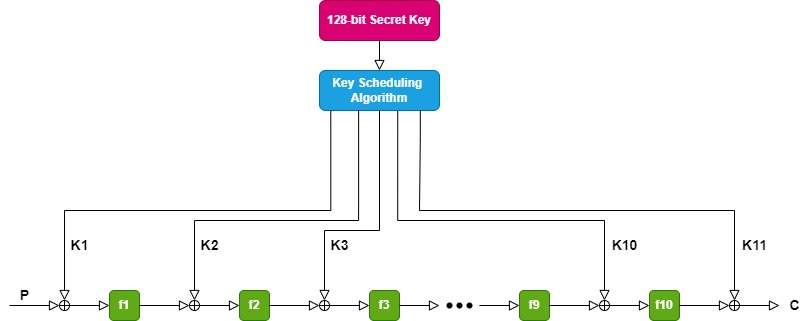
\includegraphics[width=17cm]{AES-128 (1).jpg}\vspace{10.5cm}\\
		\textbf{THE END}
	\end{center}
	
\end{document}